\section{Asset Tokenisation}
\label{sec:asset_tokenisation}
Asset tokenization is the process of converting the rights to a physical or intangible asset into a digital token on a blockchain. These tokens can represent a wide variety of financial instruments, including equities, bonds, real estate, commodities, and even artworks or intellectual property. There are several types of tokens, each with their unique properties and applications \cite{isda_tokenisation_models}. Table \ref{tab:tokenisation_models} provides a breakdown of the distinguishing features of each model.

\begin{itemize}

    \item \textbf{Registered Tokens} \citep{registered_tokens}. These tokens have an identity layer. Ownership of these tokens is tied to a specific identity, which can be verified against a registry. This is particularly useful for assets where legal and regulatory compliance is crucial (Figure \ref{subfig:registered}). The first ever digital bond, denominated in GBP, issued by the European Investment Bank lies in this category \citep{eib_bond}.

    In the Registered model, ownership of tokenised assets is tied to a specific identity stored in a register controlled by a \textit{Registrar} entity. The Registrar and the \textit{Issuer} of the tokens could coincide. When they do not, the Issuer submits instructions to the Registrar when issuance operations have to be performed, as well as transferring the ownership rights of the tokenised securities to the Participants in the network. Transfer operations are performed by the Participants by issuing transfer instructions to the Registrar. It is important to highlight the fact that in this scenario the power to update and rectify entries in the registers lies exclusively with the \textit{Registrar}, the Issuers and Participants can simply communicate the actions they want to perform. Another important aspect to consider is that in this scenario the tokens merely represent evidence of rights, they are not assets in their own right, and modifying the state of the register simply involves updating the token balances of specific participants. Note that two registers are present: the first, on-chain register stores the mapping between public keys and tokens, i.e. the holding relationships; the second, off-chain register maps public keys to real-world identities. The Registrar also keeps an offline business continuity record, essentially replicating the on-chain records, to ensure operations can proceed in case of network disruptions.
    
    \item \textbf{Bearer Tokens} \citep{bearer_tokens}. These are tokens that grant ownership to whoever holds them, much like cash or certain types of bonds. They don't have an embedded identity layer that verifies the owner's identity. Whoever controls the private key controls the asset (Figure \ref{subfig:bearer}). Stablecoins (dollar-pedgged digital coins) such as USDT \citep{usdt} and USDC \citep{usdc} fall into this category.

    In the Bearer model, the tokens are intangible assets in their own right and ownership of tokenised assets relies exclusively on the control of the tokens themselves. In this scenario, no Registrar is needed; the Issuer simply creates the tokens and transfers ownership to the Participants, which are then fully responsible for administering the assets. It is important to highlight that in this scenario the token holder has exclusive control, meaning the token holder has additional operational burdens as well as increased exposure to risk. Moving funds requires updating ownership of the asset themselves (meaning that once the asset is transferred, associated rights and control over it now belong to the new holder, increasing risks related to irreversibility of transactions in case of errors).

    \item \textbf{Claim Tokens} \citep{claims_tokens}. These tokens represent a claim or a right against an asset, rather than the asset itself. They're often used in debt issuance or other types of contractual agreements where one party has a claim against another (Figure \ref{subfig:claims}) The Depository Trust \& Clearing Corporation's (DTCC) Ion Project, a blockchain-based alternative settlement engine, falls into this category \citep{project_ion}.

    In the Claims model, a third-party Operator is responsible for running and maintaining the blockchain system, while also providing the rules for operating within the system. The Claims model resembles the Registered model, however we note a few key differences. Firstly, there is no additional identity layer, ownership is fully determined within the boundaries of the blockchain system by means of cryptography (mapping between public keys and token representations). Secondly, the Issuer and Operator cannot coincide: the Issuer is exclusively responsible for granting ownership rights to the Participant while the Operator's only responsibility is to run the network. Lastly, Participants are directly interacting with each other: ownership changes are still reflected by updates to a ledger of balances, however these are performed directly by Participants by interacting with smart contracts deployed by the Operator (and whose specifications are defined in the system rules). Overall, the Claims model is more flexible than the Registered model in the array of underlying assets it can represent, however this also introduces an extra layer of complexity as the claims must be exercised through appropriate legal channels and contractual arrangements.
    
\end{itemize}


\begin{figure}
     \centering
     \begin{subfigure}[b]{0.8\textwidth}
         \centering
         \begin{minipage}[b][8cm][c]{\linewidth} % Adjust the height (4.5cm) as needed
             \centering
             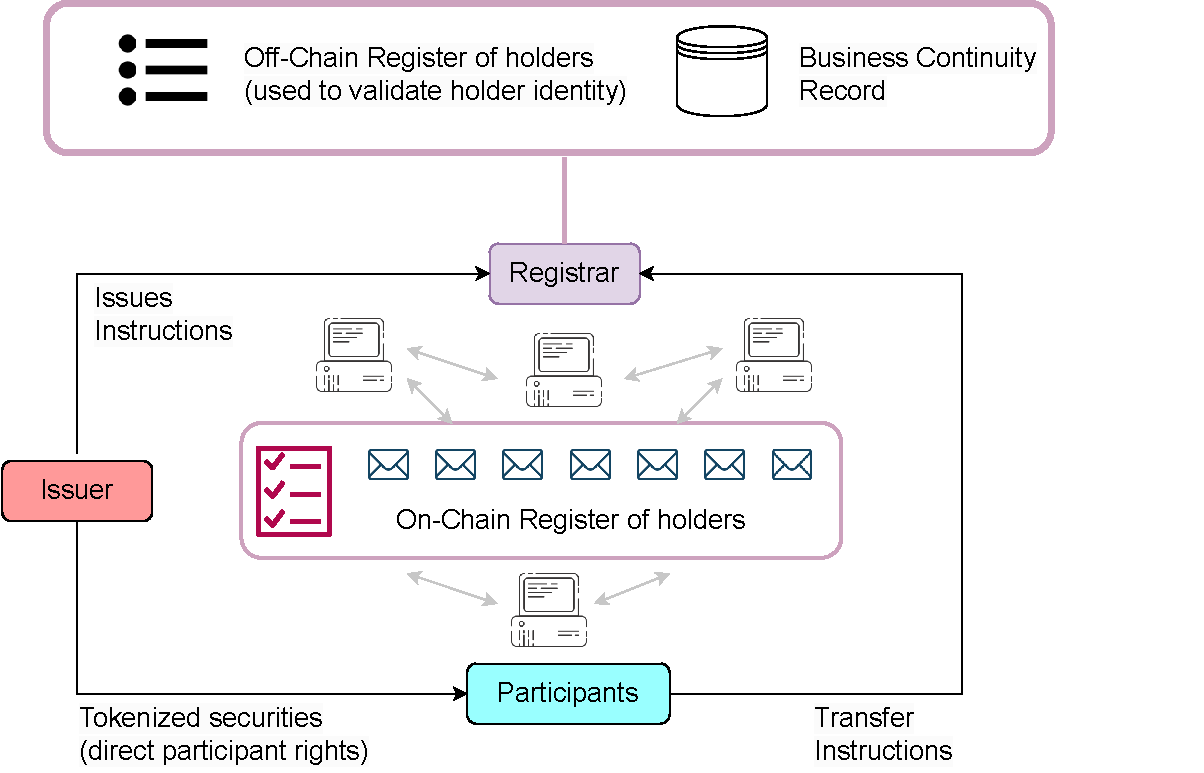
\includegraphics[width=0.8\linewidth]{images/chapter-2/registerd_custom.drawio.pdf}
             \caption{Registered}
             \label{subfig:registered}
         \end{minipage}
     \end{subfigure}
     \\
     \begin{subfigure}[b]{0.7\textwidth}
         \centering
         \begin{minipage}[b][8cm][c]{\linewidth} % Adjust the height (4.5cm) as needed
             \centering
             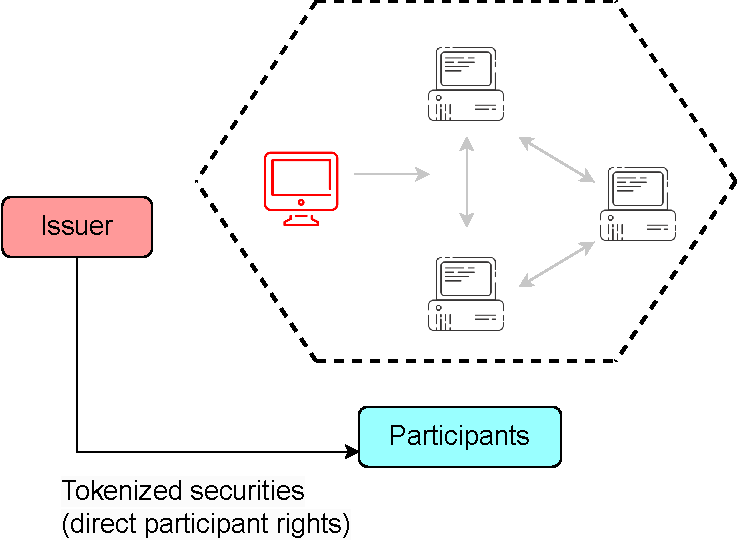
\includegraphics[width=0.8\linewidth]{images/chapter-2/bearer_custom.drawio.pdf}
             \caption{Bearer}
             \label{subfig:bearer}
         \end{minipage}
     \end{subfigure}
     \\
     \begin{subfigure}[b]{0.7\textwidth}
         \centering
         \begin{minipage}[b][7cm][c]{\linewidth} % Adjust the height (4.5cm) as needed
             \centering
             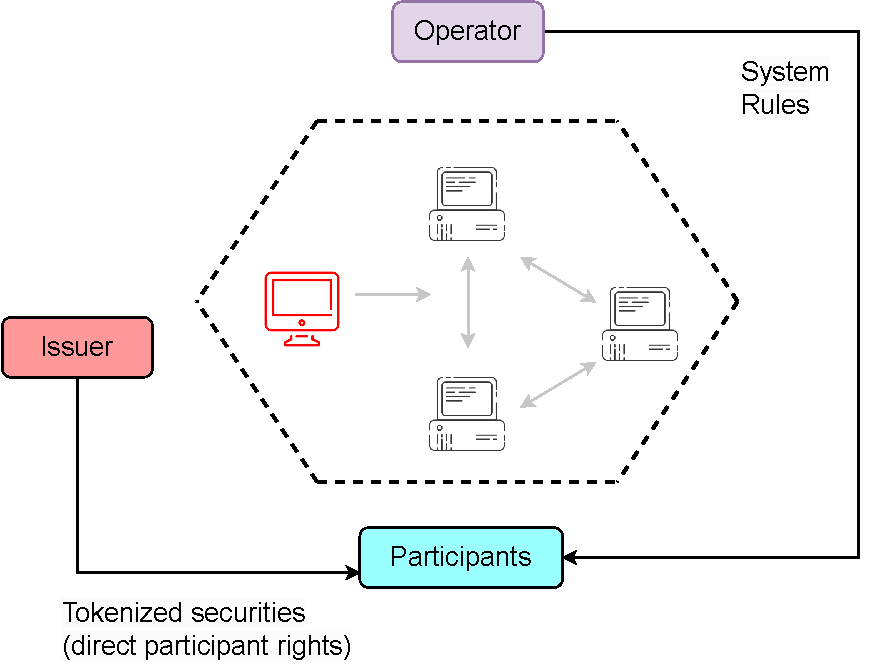
\includegraphics[width=0.8\linewidth]{images/chapter-2/claims_custom.drawio.pdf}
             \caption{Claims}
             \label{subfig:claims}
         \end{minipage}
     \end{subfigure}
    \caption[Asset tokenisation models]{Adapted from \citep{tokenovate_tokenisation_models} \footnotemark. Three asset tokenisation models showing roles of \textit{Issuers}, \textit{Registrars}, and \textit{Participants} in the network: Registered (\ref{subfig:registered}), Bearer (\ref{subfig:bearer}), and Claims (\ref{subfig:claims}) models.}
    
    \label{fig:three graphs}
\end{figure}
\footnotetext{This image is reproduced with permission from Tokenovate Ltd.}


\renewcommand\tabularxcolumn[1]{m{#1}}% for vertical centering text in X column
\begin{table}[]
    \centering

    \begin{tabularx}{\textwidth} { 
           >{\centering\arraybackslash}X 
           >{\centering\arraybackslash}X
           >{\centering\arraybackslash}X
           >{\centering\arraybackslash}X
           >{\centering\arraybackslash}X
           >{\centering\arraybackslash}X  }
         \toprule[1.5pt]
         \textit{Tokenisation Model} & \textit{Description} & \textit{Control} & \textit{Traits} & \textit{Transfer Mechanism} & \textit{Examples} \\
         \midrule[1.5pt]
         
         Registered & \vspace{10pt} Rights determined by reference to a register controlled by Registrar \vspace{1pt} & Registrar has powers to update/rectify entries & Mere data/evidence of rights & Updating token balances & First EIB \href{https://www.eib.org/en/press/all/2023-030-eib-issues-its-first-ever-digital-bond-in-british-pounds}{Digital Bond in Sterling} \citep{eib_bond} \\
    
         \hline

         Bearer & \vspace{10pt} Rights determined by reference to exclusive control of tokens \vspace{10pt} & Token holder has exclusive control & Intangible asset in its own right & Transfer of control of token & \href{https://tether.to/en/why-tether}{USDT} \citep{usdt}, \href{https://www.circle.com/en/usdc}{USDC} \citep{usdc} \\ 

         \hline

         Claims & \vspace{10pt} Rights determined by reference to entries in a system controlled by a third-party Operator \vspace{10pt} & Third-party operator has powers to update/rectify entries & Mere data/evidence of rights & Updating token balances & \href{https://www.dtcc.com/news/2022/august/22/project-ion}{DTCC Project Ion} \citep{project_ion} \\

         \bottomrule[1.5pt]

    \end{tabularx}

    \caption{Properties of different asset tokenisation models.}
    \label{tab:tokenisation_models}
\end{table}


Tokenisation has significant effects on the collateral management process:

\begin{itemize}
    \item \textbf{Enhanced Liquidity}. Tokenization essentially acts as a liquidity enhancer, particularly for assets traditionally characterized by illiquidity. Assets such as real estate, private equity, or even fine art, can be divided into fractional ownership represented by tokens. This process makes it feasible to sell or trade fractions of these assets, thereby unlocking their value and transforming them into more liquid instruments. This increase in liquidity consequently extends their functionality as collateral. The tokens can be more readily bought, sold, or valued, thereby rendering them more practical as collateral in transactions. Furthermore, their divisible nature implies that exact collateral amounts can be more effortlessly arranged, leading to improved capital utilization.
    
    \item \textbf{Operational Efficiency}. The potential efficiency gains through tokenization in collateral management are substantial. By transforming assets into digital tokens on a blockchain, the process of transferring these assets, whether for a collateral call, substitution, or release, becomes notably more efficient. The removal of intermediaries and the streamlined, automated procedures made possible by smart contracts can significantly reduce the time and cost of these transactions. This automation reduces manual errors and the overall complexity of collateral management, making it more straightforward and less resource-intensive.
    
    \item \textbf{Transparency and Auditability}. The adoption of blockchain technology in asset tokenization introduces an unprecedented level of transparency and auditability within the scope of collateral management \citep{isda_collateral_sc_legal_guidelines}. Each token transaction—be it related to a collateral call, release, or substitution—is indelibly recorded on the blockchain in an immutable ledger. Authorized parties can scrutinize this ledger to gain a transparent, auditable record of all transactions. This enhances the efficiency of risk management in collateral operations, as involved parties can easily access and evaluate the necessary data. While the immutable nature of blockchain transactions does aid in regulatory compliance, it is important to note that the technology is not a panacea for all compliance challenges. Legal texts often contain ambiguities inherent to natural language, making some rules and regulations open to interpretation. Therefore, while blockchain records can serve as strong corroborating evidence, they may not guarantee full compliance with all relevant legal requirements. Nevertheless, for rules and regulations deemed fully automatable by regulatory bodies, blockchain adds an invaluable layer of trust and security to the compliance process.

    \item \textbf{Interoperability and Flexibility}. Tokenization also brings about a new degree of interoperability and flexibility to collateral management. In a tokenized world, the same asset can exist on multiple chains, enhancing the flexibility of collateral operations. Cross-chain interoperability made possible by blockchain technology implies that collateral can be easily transferred across various platforms, catering to the diverse needs of participants in the collateral management lifecycle. This feature, however, also introduces the risk of "double use" or "double spending," where the same asset could potentially be used as collateral on multiple platforms simultaneously. To mitigate this risk, the use of decentralized identity and ownership verification systems \citep{dib2020decentralized}, smart contracts with built-in "lock-up" features \citep{token_lockup}, or cross-chain oracle services \citep{crosschain_oracles} could be implemented to track and authenticate the status of tokenized assets, ensuring they are not misused.

    \item \textbf{Democratization of Access}. Finally, tokenization potentially democratizes access to certain types of collateral. By breaking down larger, illiquid assets into smaller, more accessible tokens, a wider range of participants can be recipients of these assets for collateral use. This diversification enlarges the pool of available collateral, thereby enhancing risk mitigation by reducing overreliance on a limited set of assets.

\end{itemize}